% Created by tikzDevice version 0.12.3.1 on 2022-03-28 12:21:44
% !TEX encoding = UTF-8 Unicode
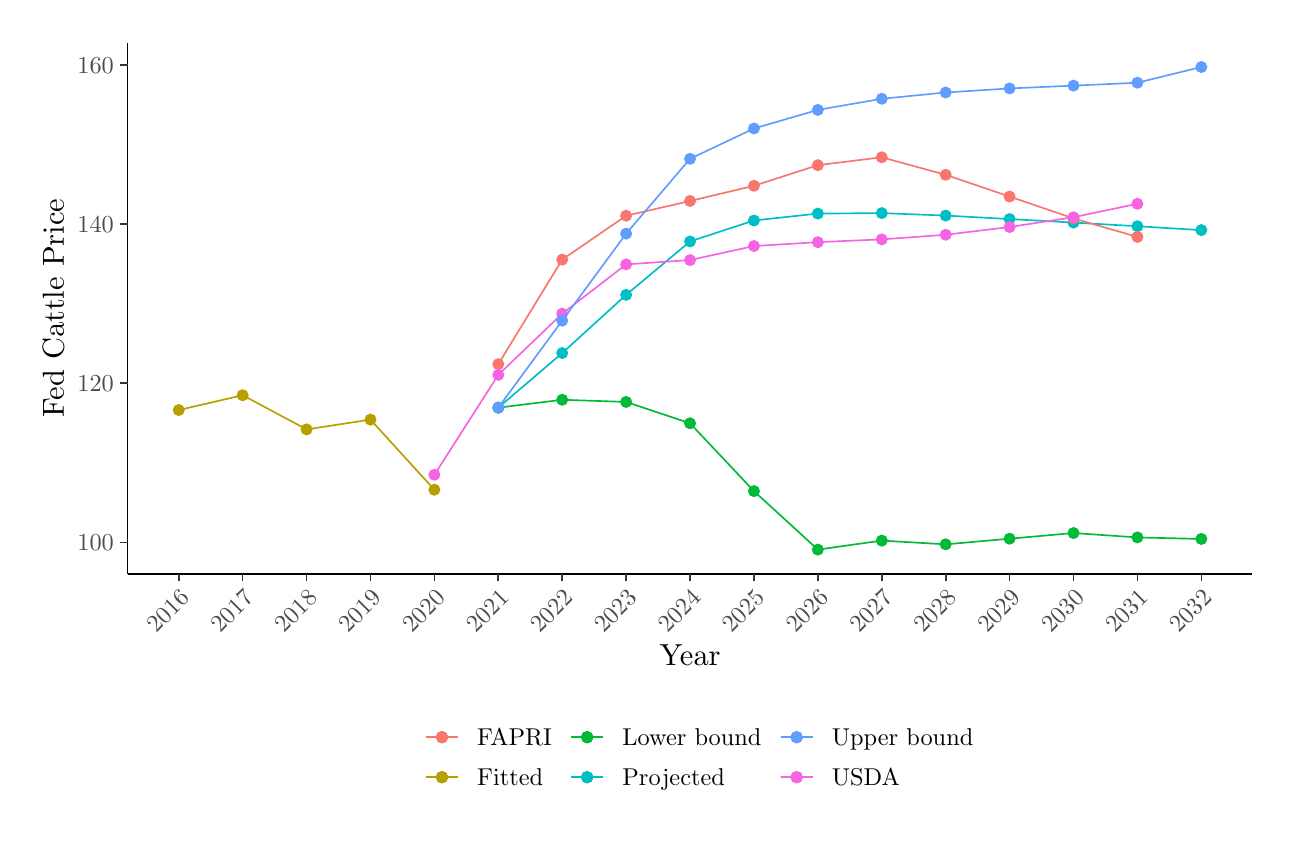
\begin{tikzpicture}[x=1pt,y=1pt]
\definecolor{fillColor}{RGB}{255,255,255}
\path[use as bounding box,fill=fillColor,fill opacity=0.00] (0,0) rectangle (448.07,289.08);
\begin{scope}
\path[clip] (  0.00,  0.00) rectangle (448.07,289.08);
\definecolor{drawColor}{RGB}{255,255,255}
\definecolor{fillColor}{RGB}{255,255,255}

\path[draw=drawColor,line width= 0.6pt,line join=round,line cap=round,fill=fillColor] (  0.00,  0.00) rectangle (448.07,289.08);
\end{scope}
\begin{scope}
\path[clip] ( 36.11, 91.76) rectangle (442.57,283.58);
\definecolor{fillColor}{RGB}{255,255,255}

\path[fill=fillColor] ( 36.11, 91.76) rectangle (442.57,283.58);
\definecolor{drawColor}{RGB}{183,159,0}

\path[draw=drawColor,line width= 0.6pt,line join=round] ( 54.59,150.91) --
	( 77.68,156.26) --
	(100.78,143.92) --
	(123.87,147.45) --
	(146.96,122.11);
\definecolor{fillColor}{RGB}{183,159,0}

\path[draw=drawColor,line width= 0.4pt,line join=round,line cap=round,fill=fillColor] ( 54.59,150.91) circle (  1.96);

\path[draw=drawColor,line width= 0.4pt,line join=round,line cap=round,fill=fillColor] ( 77.68,156.26) circle (  1.96);

\path[draw=drawColor,line width= 0.4pt,line join=round,line cap=round,fill=fillColor] (100.78,143.92) circle (  1.96);

\path[draw=drawColor,line width= 0.4pt,line join=round,line cap=round,fill=fillColor] (123.87,147.45) circle (  1.96);

\path[draw=drawColor,line width= 0.4pt,line join=round,line cap=round,fill=fillColor] (146.96,122.11) circle (  1.96);
\definecolor{drawColor}{RGB}{0,186,56}

\path[draw=drawColor,line width= 0.6pt,line join=round] (170.06,151.77) --
	(193.15,154.62) --
	(216.25,153.84) --
	(239.34,146.13) --
	(262.44,121.62) --
	(285.53,100.48) --
	(308.63,103.73) --
	(331.72,102.38) --
	(354.81,104.42) --
	(377.91,106.46) --
	(401.00,104.88) --
	(424.10,104.33);
\definecolor{fillColor}{RGB}{0,186,56}

\path[draw=drawColor,line width= 0.4pt,line join=round,line cap=round,fill=fillColor] (170.06,151.77) circle (  1.96);

\path[draw=drawColor,line width= 0.4pt,line join=round,line cap=round,fill=fillColor] (193.15,154.62) circle (  1.96);

\path[draw=drawColor,line width= 0.4pt,line join=round,line cap=round,fill=fillColor] (216.25,153.84) circle (  1.96);

\path[draw=drawColor,line width= 0.4pt,line join=round,line cap=round,fill=fillColor] (239.34,146.13) circle (  1.96);

\path[draw=drawColor,line width= 0.4pt,line join=round,line cap=round,fill=fillColor] (262.44,121.62) circle (  1.96);

\path[draw=drawColor,line width= 0.4pt,line join=round,line cap=round,fill=fillColor] (285.53,100.48) circle (  1.96);

\path[draw=drawColor,line width= 0.4pt,line join=round,line cap=round,fill=fillColor] (308.63,103.73) circle (  1.96);

\path[draw=drawColor,line width= 0.4pt,line join=round,line cap=round,fill=fillColor] (331.72,102.38) circle (  1.96);

\path[draw=drawColor,line width= 0.4pt,line join=round,line cap=round,fill=fillColor] (354.81,104.42) circle (  1.96);

\path[draw=drawColor,line width= 0.4pt,line join=round,line cap=round,fill=fillColor] (377.91,106.46) circle (  1.96);

\path[draw=drawColor,line width= 0.4pt,line join=round,line cap=round,fill=fillColor] (401.00,104.88) circle (  1.96);

\path[draw=drawColor,line width= 0.4pt,line join=round,line cap=round,fill=fillColor] (424.10,104.33) circle (  1.96);
\definecolor{drawColor}{RGB}{0,191,196}

\path[draw=drawColor,line width= 0.6pt,line join=round] (170.06,151.77) --
	(193.15,171.50) --
	(216.25,192.53) --
	(239.34,211.83) --
	(262.44,219.40) --
	(285.53,221.90) --
	(308.63,222.07) --
	(331.72,221.18) --
	(354.81,219.92) --
	(377.91,218.65) --
	(401.00,217.33) --
	(424.10,215.92);
\definecolor{fillColor}{RGB}{0,191,196}

\path[draw=drawColor,line width= 0.4pt,line join=round,line cap=round,fill=fillColor] (170.06,151.77) circle (  1.96);

\path[draw=drawColor,line width= 0.4pt,line join=round,line cap=round,fill=fillColor] (193.15,171.50) circle (  1.96);

\path[draw=drawColor,line width= 0.4pt,line join=round,line cap=round,fill=fillColor] (216.25,192.53) circle (  1.96);

\path[draw=drawColor,line width= 0.4pt,line join=round,line cap=round,fill=fillColor] (239.34,211.83) circle (  1.96);

\path[draw=drawColor,line width= 0.4pt,line join=round,line cap=round,fill=fillColor] (262.44,219.40) circle (  1.96);

\path[draw=drawColor,line width= 0.4pt,line join=round,line cap=round,fill=fillColor] (285.53,221.90) circle (  1.96);

\path[draw=drawColor,line width= 0.4pt,line join=round,line cap=round,fill=fillColor] (308.63,222.07) circle (  1.96);

\path[draw=drawColor,line width= 0.4pt,line join=round,line cap=round,fill=fillColor] (331.72,221.18) circle (  1.96);

\path[draw=drawColor,line width= 0.4pt,line join=round,line cap=round,fill=fillColor] (354.81,219.92) circle (  1.96);

\path[draw=drawColor,line width= 0.4pt,line join=round,line cap=round,fill=fillColor] (377.91,218.65) circle (  1.96);

\path[draw=drawColor,line width= 0.4pt,line join=round,line cap=round,fill=fillColor] (401.00,217.33) circle (  1.96);

\path[draw=drawColor,line width= 0.4pt,line join=round,line cap=round,fill=fillColor] (424.10,215.92) circle (  1.96);
\definecolor{drawColor}{RGB}{248,118,109}

\path[draw=drawColor,line width= 0.6pt,line join=round] (170.06,167.48) --
	(193.15,205.27) --
	(216.25,221.13) --
	(239.34,226.45) --
	(262.44,231.94) --
	(285.53,239.39) --
	(308.63,242.24) --
	(331.72,235.91) --
	(354.81,228.06) --
	(377.91,220.15) --
	(401.00,213.47);
\definecolor{fillColor}{RGB}{248,118,109}

\path[draw=drawColor,line width= 0.4pt,line join=round,line cap=round,fill=fillColor] (170.06,167.48) circle (  1.96);

\path[draw=drawColor,line width= 0.4pt,line join=round,line cap=round,fill=fillColor] (193.15,205.27) circle (  1.96);

\path[draw=drawColor,line width= 0.4pt,line join=round,line cap=round,fill=fillColor] (216.25,221.13) circle (  1.96);

\path[draw=drawColor,line width= 0.4pt,line join=round,line cap=round,fill=fillColor] (239.34,226.45) circle (  1.96);

\path[draw=drawColor,line width= 0.4pt,line join=round,line cap=round,fill=fillColor] (262.44,231.94) circle (  1.96);

\path[draw=drawColor,line width= 0.4pt,line join=round,line cap=round,fill=fillColor] (285.53,239.39) circle (  1.96);

\path[draw=drawColor,line width= 0.4pt,line join=round,line cap=round,fill=fillColor] (308.63,242.24) circle (  1.96);

\path[draw=drawColor,line width= 0.4pt,line join=round,line cap=round,fill=fillColor] (331.72,235.91) circle (  1.96);

\path[draw=drawColor,line width= 0.4pt,line join=round,line cap=round,fill=fillColor] (354.81,228.06) circle (  1.96);

\path[draw=drawColor,line width= 0.4pt,line join=round,line cap=round,fill=fillColor] (377.91,220.15) circle (  1.96);

\path[draw=drawColor,line width= 0.4pt,line join=round,line cap=round,fill=fillColor] (401.00,213.47) circle (  1.96);
\definecolor{drawColor}{RGB}{245,100,227}

\path[draw=drawColor,line width= 0.6pt,line join=round] (146.96,127.52) --
	(170.06,163.62) --
	(193.15,185.74) --
	(216.25,203.55) --
	(239.34,205.10) --
	(262.44,210.17) --
	(285.53,211.57) --
	(308.63,212.58) --
	(331.72,214.25) --
	(354.81,217.04) --
	(377.91,220.58) --
	(401.00,225.44);
\definecolor{fillColor}{RGB}{245,100,227}

\path[draw=drawColor,line width= 0.4pt,line join=round,line cap=round,fill=fillColor] (146.96,127.52) circle (  1.96);

\path[draw=drawColor,line width= 0.4pt,line join=round,line cap=round,fill=fillColor] (170.06,163.62) circle (  1.96);

\path[draw=drawColor,line width= 0.4pt,line join=round,line cap=round,fill=fillColor] (193.15,185.74) circle (  1.96);

\path[draw=drawColor,line width= 0.4pt,line join=round,line cap=round,fill=fillColor] (216.25,203.55) circle (  1.96);

\path[draw=drawColor,line width= 0.4pt,line join=round,line cap=round,fill=fillColor] (239.34,205.10) circle (  1.96);

\path[draw=drawColor,line width= 0.4pt,line join=round,line cap=round,fill=fillColor] (262.44,210.17) circle (  1.96);

\path[draw=drawColor,line width= 0.4pt,line join=round,line cap=round,fill=fillColor] (285.53,211.57) circle (  1.96);

\path[draw=drawColor,line width= 0.4pt,line join=round,line cap=round,fill=fillColor] (308.63,212.58) circle (  1.96);

\path[draw=drawColor,line width= 0.4pt,line join=round,line cap=round,fill=fillColor] (331.72,214.25) circle (  1.96);

\path[draw=drawColor,line width= 0.4pt,line join=round,line cap=round,fill=fillColor] (354.81,217.04) circle (  1.96);

\path[draw=drawColor,line width= 0.4pt,line join=round,line cap=round,fill=fillColor] (377.91,220.58) circle (  1.96);

\path[draw=drawColor,line width= 0.4pt,line join=round,line cap=round,fill=fillColor] (401.00,225.44) circle (  1.96);
\definecolor{drawColor}{RGB}{97,156,255}

\path[draw=drawColor,line width= 0.6pt,line join=round] (170.06,151.77) --
	(193.15,183.21) --
	(216.25,214.65) --
	(239.34,241.69) --
	(262.44,252.65) --
	(285.53,259.36) --
	(308.63,263.38) --
	(331.72,265.66) --
	(354.81,267.12) --
	(377.91,268.13) --
	(401.00,269.19) --
	(424.10,274.86);
\definecolor{fillColor}{RGB}{97,156,255}

\path[draw=drawColor,line width= 0.4pt,line join=round,line cap=round,fill=fillColor] (170.06,151.77) circle (  1.96);

\path[draw=drawColor,line width= 0.4pt,line join=round,line cap=round,fill=fillColor] (193.15,183.21) circle (  1.96);

\path[draw=drawColor,line width= 0.4pt,line join=round,line cap=round,fill=fillColor] (216.25,214.65) circle (  1.96);

\path[draw=drawColor,line width= 0.4pt,line join=round,line cap=round,fill=fillColor] (239.34,241.69) circle (  1.96);

\path[draw=drawColor,line width= 0.4pt,line join=round,line cap=round,fill=fillColor] (262.44,252.65) circle (  1.96);

\path[draw=drawColor,line width= 0.4pt,line join=round,line cap=round,fill=fillColor] (285.53,259.36) circle (  1.96);

\path[draw=drawColor,line width= 0.4pt,line join=round,line cap=round,fill=fillColor] (308.63,263.38) circle (  1.96);

\path[draw=drawColor,line width= 0.4pt,line join=round,line cap=round,fill=fillColor] (331.72,265.66) circle (  1.96);

\path[draw=drawColor,line width= 0.4pt,line join=round,line cap=round,fill=fillColor] (354.81,267.12) circle (  1.96);

\path[draw=drawColor,line width= 0.4pt,line join=round,line cap=round,fill=fillColor] (377.91,268.13) circle (  1.96);

\path[draw=drawColor,line width= 0.4pt,line join=round,line cap=round,fill=fillColor] (401.00,269.19) circle (  1.96);

\path[draw=drawColor,line width= 0.4pt,line join=round,line cap=round,fill=fillColor] (424.10,274.86) circle (  1.96);
\end{scope}
\begin{scope}
\path[clip] (  0.00,  0.00) rectangle (448.07,289.08);
\definecolor{drawColor}{RGB}{0,0,0}

\path[draw=drawColor,line width= 0.6pt,line join=round] ( 36.11, 91.76) --
	( 36.11,283.58);
\end{scope}
\begin{scope}
\path[clip] (  0.00,  0.00) rectangle (448.07,289.08);
\definecolor{drawColor}{gray}{0.30}

\node[text=drawColor,anchor=base east,inner sep=0pt, outer sep=0pt, scale=  0.88] at ( 31.16,100.01) {100};

\node[text=drawColor,anchor=base east,inner sep=0pt, outer sep=0pt, scale=  0.88] at ( 31.16,157.54) {120};

\node[text=drawColor,anchor=base east,inner sep=0pt, outer sep=0pt, scale=  0.88] at ( 31.16,215.07) {140};

\node[text=drawColor,anchor=base east,inner sep=0pt, outer sep=0pt, scale=  0.88] at ( 31.16,272.61) {160};
\end{scope}
\begin{scope}
\path[clip] (  0.00,  0.00) rectangle (448.07,289.08);
\definecolor{drawColor}{gray}{0.20}

\path[draw=drawColor,line width= 0.6pt,line join=round] ( 33.36,103.04) --
	( 36.11,103.04);

\path[draw=drawColor,line width= 0.6pt,line join=round] ( 33.36,160.57) --
	( 36.11,160.57);

\path[draw=drawColor,line width= 0.6pt,line join=round] ( 33.36,218.10) --
	( 36.11,218.10);

\path[draw=drawColor,line width= 0.6pt,line join=round] ( 33.36,275.64) --
	( 36.11,275.64);
\end{scope}
\begin{scope}
\path[clip] (  0.00,  0.00) rectangle (448.07,289.08);
\definecolor{drawColor}{RGB}{0,0,0}

\path[draw=drawColor,line width= 0.6pt,line join=round] ( 36.11, 91.76) --
	(442.57, 91.76);
\end{scope}
\begin{scope}
\path[clip] (  0.00,  0.00) rectangle (448.07,289.08);
\definecolor{drawColor}{gray}{0.20}

\path[draw=drawColor,line width= 0.6pt,line join=round] ( 54.59, 89.01) --
	( 54.59, 91.76);

\path[draw=drawColor,line width= 0.6pt,line join=round] ( 77.68, 89.01) --
	( 77.68, 91.76);

\path[draw=drawColor,line width= 0.6pt,line join=round] (100.78, 89.01) --
	(100.78, 91.76);

\path[draw=drawColor,line width= 0.6pt,line join=round] (123.87, 89.01) --
	(123.87, 91.76);

\path[draw=drawColor,line width= 0.6pt,line join=round] (146.96, 89.01) --
	(146.96, 91.76);

\path[draw=drawColor,line width= 0.6pt,line join=round] (170.06, 89.01) --
	(170.06, 91.76);

\path[draw=drawColor,line width= 0.6pt,line join=round] (193.15, 89.01) --
	(193.15, 91.76);

\path[draw=drawColor,line width= 0.6pt,line join=round] (216.25, 89.01) --
	(216.25, 91.76);

\path[draw=drawColor,line width= 0.6pt,line join=round] (239.34, 89.01) --
	(239.34, 91.76);

\path[draw=drawColor,line width= 0.6pt,line join=round] (262.44, 89.01) --
	(262.44, 91.76);

\path[draw=drawColor,line width= 0.6pt,line join=round] (285.53, 89.01) --
	(285.53, 91.76);

\path[draw=drawColor,line width= 0.6pt,line join=round] (308.63, 89.01) --
	(308.63, 91.76);

\path[draw=drawColor,line width= 0.6pt,line join=round] (331.72, 89.01) --
	(331.72, 91.76);

\path[draw=drawColor,line width= 0.6pt,line join=round] (354.81, 89.01) --
	(354.81, 91.76);

\path[draw=drawColor,line width= 0.6pt,line join=round] (377.91, 89.01) --
	(377.91, 91.76);

\path[draw=drawColor,line width= 0.6pt,line join=round] (401.00, 89.01) --
	(401.00, 91.76);

\path[draw=drawColor,line width= 0.6pt,line join=round] (424.10, 89.01) --
	(424.10, 91.76);
\end{scope}
\begin{scope}
\path[clip] (  0.00,  0.00) rectangle (448.07,289.08);
\definecolor{drawColor}{gray}{0.30}

\node[text=drawColor,rotate= 45.00,anchor=base east,inner sep=0pt, outer sep=0pt, scale=  0.88] at ( 58.87, 82.52) {2016};

\node[text=drawColor,rotate= 45.00,anchor=base east,inner sep=0pt, outer sep=0pt, scale=  0.88] at ( 81.97, 82.52) {2017};

\node[text=drawColor,rotate= 45.00,anchor=base east,inner sep=0pt, outer sep=0pt, scale=  0.88] at (105.06, 82.52) {2018};

\node[text=drawColor,rotate= 45.00,anchor=base east,inner sep=0pt, outer sep=0pt, scale=  0.88] at (128.16, 82.52) {2019};

\node[text=drawColor,rotate= 45.00,anchor=base east,inner sep=0pt, outer sep=0pt, scale=  0.88] at (151.25, 82.52) {2020};

\node[text=drawColor,rotate= 45.00,anchor=base east,inner sep=0pt, outer sep=0pt, scale=  0.88] at (174.34, 82.52) {2021};

\node[text=drawColor,rotate= 45.00,anchor=base east,inner sep=0pt, outer sep=0pt, scale=  0.88] at (197.44, 82.52) {2022};

\node[text=drawColor,rotate= 45.00,anchor=base east,inner sep=0pt, outer sep=0pt, scale=  0.88] at (220.53, 82.52) {2023};

\node[text=drawColor,rotate= 45.00,anchor=base east,inner sep=0pt, outer sep=0pt, scale=  0.88] at (243.63, 82.52) {2024};

\node[text=drawColor,rotate= 45.00,anchor=base east,inner sep=0pt, outer sep=0pt, scale=  0.88] at (266.72, 82.52) {2025};

\node[text=drawColor,rotate= 45.00,anchor=base east,inner sep=0pt, outer sep=0pt, scale=  0.88] at (289.82, 82.52) {2026};

\node[text=drawColor,rotate= 45.00,anchor=base east,inner sep=0pt, outer sep=0pt, scale=  0.88] at (312.91, 82.52) {2027};

\node[text=drawColor,rotate= 45.00,anchor=base east,inner sep=0pt, outer sep=0pt, scale=  0.88] at (336.01, 82.52) {2028};

\node[text=drawColor,rotate= 45.00,anchor=base east,inner sep=0pt, outer sep=0pt, scale=  0.88] at (359.10, 82.52) {2029};

\node[text=drawColor,rotate= 45.00,anchor=base east,inner sep=0pt, outer sep=0pt, scale=  0.88] at (382.20, 82.52) {2030};

\node[text=drawColor,rotate= 45.00,anchor=base east,inner sep=0pt, outer sep=0pt, scale=  0.88] at (405.29, 82.52) {2031};

\node[text=drawColor,rotate= 45.00,anchor=base east,inner sep=0pt, outer sep=0pt, scale=  0.88] at (428.38, 82.52) {2032};
\end{scope}
\begin{scope}
\path[clip] (  0.00,  0.00) rectangle (448.07,289.08);
\definecolor{drawColor}{RGB}{0,0,0}

\node[text=drawColor,anchor=base,inner sep=0pt, outer sep=0pt, scale=  1.10] at (239.34, 58.55) {Year};
\end{scope}
\begin{scope}
\path[clip] (  0.00,  0.00) rectangle (448.07,289.08);
\definecolor{drawColor}{RGB}{0,0,0}

\node[text=drawColor,rotate= 90.00,anchor=base,inner sep=0pt, outer sep=0pt, scale=  1.10] at ( 13.08,187.67) {Fed Cattle Price};
\end{scope}
\begin{scope}
\path[clip] (  0.00,  0.00) rectangle (448.07,289.08);
\definecolor{fillColor}{RGB}{255,255,255}

\path[fill=fillColor] (131.49,  5.50) rectangle (347.20, 45.41);
\end{scope}
\begin{scope}
\path[clip] (  0.00,  0.00) rectangle (448.07,289.08);
\definecolor{drawColor}{RGB}{248,118,109}

\path[draw=drawColor,line width= 0.6pt,line join=round] (143.93, 32.68) -- (155.49, 32.68);
\end{scope}
\begin{scope}
\path[clip] (  0.00,  0.00) rectangle (448.07,289.08);
\definecolor{drawColor}{RGB}{248,118,109}
\definecolor{fillColor}{RGB}{248,118,109}

\path[draw=drawColor,line width= 0.4pt,line join=round,line cap=round,fill=fillColor] (149.71, 32.68) circle (  1.96);
\end{scope}
\begin{scope}
\path[clip] (  0.00,  0.00) rectangle (448.07,289.08);
\definecolor{drawColor}{RGB}{248,118,109}

\path[draw=drawColor,line width= 0.6pt,line join=round] (143.93, 32.68) -- (155.49, 32.68);
\end{scope}
\begin{scope}
\path[clip] (  0.00,  0.00) rectangle (448.07,289.08);
\definecolor{drawColor}{RGB}{248,118,109}
\definecolor{fillColor}{RGB}{248,118,109}

\path[draw=drawColor,line width= 0.4pt,line join=round,line cap=round,fill=fillColor] (149.71, 32.68) circle (  1.96);
\end{scope}
\begin{scope}
\path[clip] (  0.00,  0.00) rectangle (448.07,289.08);
\definecolor{drawColor}{RGB}{248,118,109}

\path[draw=drawColor,line width= 0.6pt,line join=round] (143.93, 32.68) -- (155.49, 32.68);
\end{scope}
\begin{scope}
\path[clip] (  0.00,  0.00) rectangle (448.07,289.08);
\definecolor{drawColor}{RGB}{248,118,109}
\definecolor{fillColor}{RGB}{248,118,109}

\path[draw=drawColor,line width= 0.4pt,line join=round,line cap=round,fill=fillColor] (149.71, 32.68) circle (  1.96);
\end{scope}
\begin{scope}
\path[clip] (  0.00,  0.00) rectangle (448.07,289.08);
\definecolor{drawColor}{RGB}{248,118,109}

\path[draw=drawColor,line width= 0.6pt,line join=round] (143.93, 32.68) -- (155.49, 32.68);
\end{scope}
\begin{scope}
\path[clip] (  0.00,  0.00) rectangle (448.07,289.08);
\definecolor{drawColor}{RGB}{248,118,109}
\definecolor{fillColor}{RGB}{248,118,109}

\path[draw=drawColor,line width= 0.4pt,line join=round,line cap=round,fill=fillColor] (149.71, 32.68) circle (  1.96);
\end{scope}
\begin{scope}
\path[clip] (  0.00,  0.00) rectangle (448.07,289.08);
\definecolor{drawColor}{RGB}{248,118,109}

\path[draw=drawColor,line width= 0.6pt,line join=round] (143.93, 32.68) -- (155.49, 32.68);
\end{scope}
\begin{scope}
\path[clip] (  0.00,  0.00) rectangle (448.07,289.08);
\definecolor{drawColor}{RGB}{248,118,109}
\definecolor{fillColor}{RGB}{248,118,109}

\path[draw=drawColor,line width= 0.4pt,line join=round,line cap=round,fill=fillColor] (149.71, 32.68) circle (  1.96);
\end{scope}
\begin{scope}
\path[clip] (  0.00,  0.00) rectangle (448.07,289.08);
\definecolor{drawColor}{RGB}{248,118,109}

\path[draw=drawColor,line width= 0.6pt,line join=round] (143.93, 32.68) -- (155.49, 32.68);
\end{scope}
\begin{scope}
\path[clip] (  0.00,  0.00) rectangle (448.07,289.08);
\definecolor{drawColor}{RGB}{248,118,109}
\definecolor{fillColor}{RGB}{248,118,109}

\path[draw=drawColor,line width= 0.4pt,line join=round,line cap=round,fill=fillColor] (149.71, 32.68) circle (  1.96);
\end{scope}
\begin{scope}
\path[clip] (  0.00,  0.00) rectangle (448.07,289.08);
\definecolor{drawColor}{RGB}{183,159,0}

\path[draw=drawColor,line width= 0.6pt,line join=round] (143.93, 18.23) -- (155.49, 18.23);
\end{scope}
\begin{scope}
\path[clip] (  0.00,  0.00) rectangle (448.07,289.08);
\definecolor{drawColor}{RGB}{183,159,0}
\definecolor{fillColor}{RGB}{183,159,0}

\path[draw=drawColor,line width= 0.4pt,line join=round,line cap=round,fill=fillColor] (149.71, 18.23) circle (  1.96);
\end{scope}
\begin{scope}
\path[clip] (  0.00,  0.00) rectangle (448.07,289.08);
\definecolor{drawColor}{RGB}{183,159,0}

\path[draw=drawColor,line width= 0.6pt,line join=round] (143.93, 18.23) -- (155.49, 18.23);
\end{scope}
\begin{scope}
\path[clip] (  0.00,  0.00) rectangle (448.07,289.08);
\definecolor{drawColor}{RGB}{183,159,0}
\definecolor{fillColor}{RGB}{183,159,0}

\path[draw=drawColor,line width= 0.4pt,line join=round,line cap=round,fill=fillColor] (149.71, 18.23) circle (  1.96);
\end{scope}
\begin{scope}
\path[clip] (  0.00,  0.00) rectangle (448.07,289.08);
\definecolor{drawColor}{RGB}{183,159,0}

\path[draw=drawColor,line width= 0.6pt,line join=round] (143.93, 18.23) -- (155.49, 18.23);
\end{scope}
\begin{scope}
\path[clip] (  0.00,  0.00) rectangle (448.07,289.08);
\definecolor{drawColor}{RGB}{183,159,0}
\definecolor{fillColor}{RGB}{183,159,0}

\path[draw=drawColor,line width= 0.4pt,line join=round,line cap=round,fill=fillColor] (149.71, 18.23) circle (  1.96);
\end{scope}
\begin{scope}
\path[clip] (  0.00,  0.00) rectangle (448.07,289.08);
\definecolor{drawColor}{RGB}{183,159,0}

\path[draw=drawColor,line width= 0.6pt,line join=round] (143.93, 18.23) -- (155.49, 18.23);
\end{scope}
\begin{scope}
\path[clip] (  0.00,  0.00) rectangle (448.07,289.08);
\definecolor{drawColor}{RGB}{183,159,0}
\definecolor{fillColor}{RGB}{183,159,0}

\path[draw=drawColor,line width= 0.4pt,line join=round,line cap=round,fill=fillColor] (149.71, 18.23) circle (  1.96);
\end{scope}
\begin{scope}
\path[clip] (  0.00,  0.00) rectangle (448.07,289.08);
\definecolor{drawColor}{RGB}{183,159,0}

\path[draw=drawColor,line width= 0.6pt,line join=round] (143.93, 18.23) -- (155.49, 18.23);
\end{scope}
\begin{scope}
\path[clip] (  0.00,  0.00) rectangle (448.07,289.08);
\definecolor{drawColor}{RGB}{183,159,0}
\definecolor{fillColor}{RGB}{183,159,0}

\path[draw=drawColor,line width= 0.4pt,line join=round,line cap=round,fill=fillColor] (149.71, 18.23) circle (  1.96);
\end{scope}
\begin{scope}
\path[clip] (  0.00,  0.00) rectangle (448.07,289.08);
\definecolor{drawColor}{RGB}{183,159,0}

\path[draw=drawColor,line width= 0.6pt,line join=round] (143.93, 18.23) -- (155.49, 18.23);
\end{scope}
\begin{scope}
\path[clip] (  0.00,  0.00) rectangle (448.07,289.08);
\definecolor{drawColor}{RGB}{183,159,0}
\definecolor{fillColor}{RGB}{183,159,0}

\path[draw=drawColor,line width= 0.4pt,line join=round,line cap=round,fill=fillColor] (149.71, 18.23) circle (  1.96);
\end{scope}
\begin{scope}
\path[clip] (  0.00,  0.00) rectangle (448.07,289.08);
\definecolor{drawColor}{RGB}{0,186,56}

\path[draw=drawColor,line width= 0.6pt,line join=round] (196.39, 32.68) -- (207.95, 32.68);
\end{scope}
\begin{scope}
\path[clip] (  0.00,  0.00) rectangle (448.07,289.08);
\definecolor{drawColor}{RGB}{0,186,56}
\definecolor{fillColor}{RGB}{0,186,56}

\path[draw=drawColor,line width= 0.4pt,line join=round,line cap=round,fill=fillColor] (202.17, 32.68) circle (  1.96);
\end{scope}
\begin{scope}
\path[clip] (  0.00,  0.00) rectangle (448.07,289.08);
\definecolor{drawColor}{RGB}{0,186,56}

\path[draw=drawColor,line width= 0.6pt,line join=round] (196.39, 32.68) -- (207.95, 32.68);
\end{scope}
\begin{scope}
\path[clip] (  0.00,  0.00) rectangle (448.07,289.08);
\definecolor{drawColor}{RGB}{0,186,56}
\definecolor{fillColor}{RGB}{0,186,56}

\path[draw=drawColor,line width= 0.4pt,line join=round,line cap=round,fill=fillColor] (202.17, 32.68) circle (  1.96);
\end{scope}
\begin{scope}
\path[clip] (  0.00,  0.00) rectangle (448.07,289.08);
\definecolor{drawColor}{RGB}{0,186,56}

\path[draw=drawColor,line width= 0.6pt,line join=round] (196.39, 32.68) -- (207.95, 32.68);
\end{scope}
\begin{scope}
\path[clip] (  0.00,  0.00) rectangle (448.07,289.08);
\definecolor{drawColor}{RGB}{0,186,56}
\definecolor{fillColor}{RGB}{0,186,56}

\path[draw=drawColor,line width= 0.4pt,line join=round,line cap=round,fill=fillColor] (202.17, 32.68) circle (  1.96);
\end{scope}
\begin{scope}
\path[clip] (  0.00,  0.00) rectangle (448.07,289.08);
\definecolor{drawColor}{RGB}{0,186,56}

\path[draw=drawColor,line width= 0.6pt,line join=round] (196.39, 32.68) -- (207.95, 32.68);
\end{scope}
\begin{scope}
\path[clip] (  0.00,  0.00) rectangle (448.07,289.08);
\definecolor{drawColor}{RGB}{0,186,56}
\definecolor{fillColor}{RGB}{0,186,56}

\path[draw=drawColor,line width= 0.4pt,line join=round,line cap=round,fill=fillColor] (202.17, 32.68) circle (  1.96);
\end{scope}
\begin{scope}
\path[clip] (  0.00,  0.00) rectangle (448.07,289.08);
\definecolor{drawColor}{RGB}{0,186,56}

\path[draw=drawColor,line width= 0.6pt,line join=round] (196.39, 32.68) -- (207.95, 32.68);
\end{scope}
\begin{scope}
\path[clip] (  0.00,  0.00) rectangle (448.07,289.08);
\definecolor{drawColor}{RGB}{0,186,56}
\definecolor{fillColor}{RGB}{0,186,56}

\path[draw=drawColor,line width= 0.4pt,line join=round,line cap=round,fill=fillColor] (202.17, 32.68) circle (  1.96);
\end{scope}
\begin{scope}
\path[clip] (  0.00,  0.00) rectangle (448.07,289.08);
\definecolor{drawColor}{RGB}{0,186,56}

\path[draw=drawColor,line width= 0.6pt,line join=round] (196.39, 32.68) -- (207.95, 32.68);
\end{scope}
\begin{scope}
\path[clip] (  0.00,  0.00) rectangle (448.07,289.08);
\definecolor{drawColor}{RGB}{0,186,56}
\definecolor{fillColor}{RGB}{0,186,56}

\path[draw=drawColor,line width= 0.4pt,line join=round,line cap=round,fill=fillColor] (202.17, 32.68) circle (  1.96);
\end{scope}
\begin{scope}
\path[clip] (  0.00,  0.00) rectangle (448.07,289.08);
\definecolor{drawColor}{RGB}{0,191,196}

\path[draw=drawColor,line width= 0.6pt,line join=round] (196.39, 18.23) -- (207.95, 18.23);
\end{scope}
\begin{scope}
\path[clip] (  0.00,  0.00) rectangle (448.07,289.08);
\definecolor{drawColor}{RGB}{0,191,196}
\definecolor{fillColor}{RGB}{0,191,196}

\path[draw=drawColor,line width= 0.4pt,line join=round,line cap=round,fill=fillColor] (202.17, 18.23) circle (  1.96);
\end{scope}
\begin{scope}
\path[clip] (  0.00,  0.00) rectangle (448.07,289.08);
\definecolor{drawColor}{RGB}{0,191,196}

\path[draw=drawColor,line width= 0.6pt,line join=round] (196.39, 18.23) -- (207.95, 18.23);
\end{scope}
\begin{scope}
\path[clip] (  0.00,  0.00) rectangle (448.07,289.08);
\definecolor{drawColor}{RGB}{0,191,196}
\definecolor{fillColor}{RGB}{0,191,196}

\path[draw=drawColor,line width= 0.4pt,line join=round,line cap=round,fill=fillColor] (202.17, 18.23) circle (  1.96);
\end{scope}
\begin{scope}
\path[clip] (  0.00,  0.00) rectangle (448.07,289.08);
\definecolor{drawColor}{RGB}{0,191,196}

\path[draw=drawColor,line width= 0.6pt,line join=round] (196.39, 18.23) -- (207.95, 18.23);
\end{scope}
\begin{scope}
\path[clip] (  0.00,  0.00) rectangle (448.07,289.08);
\definecolor{drawColor}{RGB}{0,191,196}
\definecolor{fillColor}{RGB}{0,191,196}

\path[draw=drawColor,line width= 0.4pt,line join=round,line cap=round,fill=fillColor] (202.17, 18.23) circle (  1.96);
\end{scope}
\begin{scope}
\path[clip] (  0.00,  0.00) rectangle (448.07,289.08);
\definecolor{drawColor}{RGB}{0,191,196}

\path[draw=drawColor,line width= 0.6pt,line join=round] (196.39, 18.23) -- (207.95, 18.23);
\end{scope}
\begin{scope}
\path[clip] (  0.00,  0.00) rectangle (448.07,289.08);
\definecolor{drawColor}{RGB}{0,191,196}
\definecolor{fillColor}{RGB}{0,191,196}

\path[draw=drawColor,line width= 0.4pt,line join=round,line cap=round,fill=fillColor] (202.17, 18.23) circle (  1.96);
\end{scope}
\begin{scope}
\path[clip] (  0.00,  0.00) rectangle (448.07,289.08);
\definecolor{drawColor}{RGB}{0,191,196}

\path[draw=drawColor,line width= 0.6pt,line join=round] (196.39, 18.23) -- (207.95, 18.23);
\end{scope}
\begin{scope}
\path[clip] (  0.00,  0.00) rectangle (448.07,289.08);
\definecolor{drawColor}{RGB}{0,191,196}
\definecolor{fillColor}{RGB}{0,191,196}

\path[draw=drawColor,line width= 0.4pt,line join=round,line cap=round,fill=fillColor] (202.17, 18.23) circle (  1.96);
\end{scope}
\begin{scope}
\path[clip] (  0.00,  0.00) rectangle (448.07,289.08);
\definecolor{drawColor}{RGB}{0,191,196}

\path[draw=drawColor,line width= 0.6pt,line join=round] (196.39, 18.23) -- (207.95, 18.23);
\end{scope}
\begin{scope}
\path[clip] (  0.00,  0.00) rectangle (448.07,289.08);
\definecolor{drawColor}{RGB}{0,191,196}
\definecolor{fillColor}{RGB}{0,191,196}

\path[draw=drawColor,line width= 0.4pt,line join=round,line cap=round,fill=fillColor] (202.17, 18.23) circle (  1.96);
\end{scope}
\begin{scope}
\path[clip] (  0.00,  0.00) rectangle (448.07,289.08);
\definecolor{drawColor}{RGB}{97,156,255}

\path[draw=drawColor,line width= 0.6pt,line join=round] (272.09, 32.68) -- (283.65, 32.68);
\end{scope}
\begin{scope}
\path[clip] (  0.00,  0.00) rectangle (448.07,289.08);
\definecolor{drawColor}{RGB}{97,156,255}
\definecolor{fillColor}{RGB}{97,156,255}

\path[draw=drawColor,line width= 0.4pt,line join=round,line cap=round,fill=fillColor] (277.87, 32.68) circle (  1.96);
\end{scope}
\begin{scope}
\path[clip] (  0.00,  0.00) rectangle (448.07,289.08);
\definecolor{drawColor}{RGB}{97,156,255}

\path[draw=drawColor,line width= 0.6pt,line join=round] (272.09, 32.68) -- (283.65, 32.68);
\end{scope}
\begin{scope}
\path[clip] (  0.00,  0.00) rectangle (448.07,289.08);
\definecolor{drawColor}{RGB}{97,156,255}
\definecolor{fillColor}{RGB}{97,156,255}

\path[draw=drawColor,line width= 0.4pt,line join=round,line cap=round,fill=fillColor] (277.87, 32.68) circle (  1.96);
\end{scope}
\begin{scope}
\path[clip] (  0.00,  0.00) rectangle (448.07,289.08);
\definecolor{drawColor}{RGB}{97,156,255}

\path[draw=drawColor,line width= 0.6pt,line join=round] (272.09, 32.68) -- (283.65, 32.68);
\end{scope}
\begin{scope}
\path[clip] (  0.00,  0.00) rectangle (448.07,289.08);
\definecolor{drawColor}{RGB}{97,156,255}
\definecolor{fillColor}{RGB}{97,156,255}

\path[draw=drawColor,line width= 0.4pt,line join=round,line cap=round,fill=fillColor] (277.87, 32.68) circle (  1.96);
\end{scope}
\begin{scope}
\path[clip] (  0.00,  0.00) rectangle (448.07,289.08);
\definecolor{drawColor}{RGB}{97,156,255}

\path[draw=drawColor,line width= 0.6pt,line join=round] (272.09, 32.68) -- (283.65, 32.68);
\end{scope}
\begin{scope}
\path[clip] (  0.00,  0.00) rectangle (448.07,289.08);
\definecolor{drawColor}{RGB}{97,156,255}
\definecolor{fillColor}{RGB}{97,156,255}

\path[draw=drawColor,line width= 0.4pt,line join=round,line cap=round,fill=fillColor] (277.87, 32.68) circle (  1.96);
\end{scope}
\begin{scope}
\path[clip] (  0.00,  0.00) rectangle (448.07,289.08);
\definecolor{drawColor}{RGB}{97,156,255}

\path[draw=drawColor,line width= 0.6pt,line join=round] (272.09, 32.68) -- (283.65, 32.68);
\end{scope}
\begin{scope}
\path[clip] (  0.00,  0.00) rectangle (448.07,289.08);
\definecolor{drawColor}{RGB}{97,156,255}
\definecolor{fillColor}{RGB}{97,156,255}

\path[draw=drawColor,line width= 0.4pt,line join=round,line cap=round,fill=fillColor] (277.87, 32.68) circle (  1.96);
\end{scope}
\begin{scope}
\path[clip] (  0.00,  0.00) rectangle (448.07,289.08);
\definecolor{drawColor}{RGB}{97,156,255}

\path[draw=drawColor,line width= 0.6pt,line join=round] (272.09, 32.68) -- (283.65, 32.68);
\end{scope}
\begin{scope}
\path[clip] (  0.00,  0.00) rectangle (448.07,289.08);
\definecolor{drawColor}{RGB}{97,156,255}
\definecolor{fillColor}{RGB}{97,156,255}

\path[draw=drawColor,line width= 0.4pt,line join=round,line cap=round,fill=fillColor] (277.87, 32.68) circle (  1.96);
\end{scope}
\begin{scope}
\path[clip] (  0.00,  0.00) rectangle (448.07,289.08);
\definecolor{drawColor}{RGB}{245,100,227}

\path[draw=drawColor,line width= 0.6pt,line join=round] (272.09, 18.23) -- (283.65, 18.23);
\end{scope}
\begin{scope}
\path[clip] (  0.00,  0.00) rectangle (448.07,289.08);
\definecolor{drawColor}{RGB}{245,100,227}
\definecolor{fillColor}{RGB}{245,100,227}

\path[draw=drawColor,line width= 0.4pt,line join=round,line cap=round,fill=fillColor] (277.87, 18.23) circle (  1.96);
\end{scope}
\begin{scope}
\path[clip] (  0.00,  0.00) rectangle (448.07,289.08);
\definecolor{drawColor}{RGB}{245,100,227}

\path[draw=drawColor,line width= 0.6pt,line join=round] (272.09, 18.23) -- (283.65, 18.23);
\end{scope}
\begin{scope}
\path[clip] (  0.00,  0.00) rectangle (448.07,289.08);
\definecolor{drawColor}{RGB}{245,100,227}
\definecolor{fillColor}{RGB}{245,100,227}

\path[draw=drawColor,line width= 0.4pt,line join=round,line cap=round,fill=fillColor] (277.87, 18.23) circle (  1.96);
\end{scope}
\begin{scope}
\path[clip] (  0.00,  0.00) rectangle (448.07,289.08);
\definecolor{drawColor}{RGB}{245,100,227}

\path[draw=drawColor,line width= 0.6pt,line join=round] (272.09, 18.23) -- (283.65, 18.23);
\end{scope}
\begin{scope}
\path[clip] (  0.00,  0.00) rectangle (448.07,289.08);
\definecolor{drawColor}{RGB}{245,100,227}
\definecolor{fillColor}{RGB}{245,100,227}

\path[draw=drawColor,line width= 0.4pt,line join=round,line cap=round,fill=fillColor] (277.87, 18.23) circle (  1.96);
\end{scope}
\begin{scope}
\path[clip] (  0.00,  0.00) rectangle (448.07,289.08);
\definecolor{drawColor}{RGB}{245,100,227}

\path[draw=drawColor,line width= 0.6pt,line join=round] (272.09, 18.23) -- (283.65, 18.23);
\end{scope}
\begin{scope}
\path[clip] (  0.00,  0.00) rectangle (448.07,289.08);
\definecolor{drawColor}{RGB}{245,100,227}
\definecolor{fillColor}{RGB}{245,100,227}

\path[draw=drawColor,line width= 0.4pt,line join=round,line cap=round,fill=fillColor] (277.87, 18.23) circle (  1.96);
\end{scope}
\begin{scope}
\path[clip] (  0.00,  0.00) rectangle (448.07,289.08);
\definecolor{drawColor}{RGB}{245,100,227}

\path[draw=drawColor,line width= 0.6pt,line join=round] (272.09, 18.23) -- (283.65, 18.23);
\end{scope}
\begin{scope}
\path[clip] (  0.00,  0.00) rectangle (448.07,289.08);
\definecolor{drawColor}{RGB}{245,100,227}
\definecolor{fillColor}{RGB}{245,100,227}

\path[draw=drawColor,line width= 0.4pt,line join=round,line cap=round,fill=fillColor] (277.87, 18.23) circle (  1.96);
\end{scope}
\begin{scope}
\path[clip] (  0.00,  0.00) rectangle (448.07,289.08);
\definecolor{drawColor}{RGB}{245,100,227}

\path[draw=drawColor,line width= 0.6pt,line join=round] (272.09, 18.23) -- (283.65, 18.23);
\end{scope}
\begin{scope}
\path[clip] (  0.00,  0.00) rectangle (448.07,289.08);
\definecolor{drawColor}{RGB}{245,100,227}
\definecolor{fillColor}{RGB}{245,100,227}

\path[draw=drawColor,line width= 0.4pt,line join=round,line cap=round,fill=fillColor] (277.87, 18.23) circle (  1.96);
\end{scope}
\begin{scope}
\path[clip] (  0.00,  0.00) rectangle (448.07,289.08);
\definecolor{drawColor}{RGB}{0,0,0}

\node[text=drawColor,anchor=base west,inner sep=0pt, outer sep=0pt, scale=  0.88] at (162.44, 29.65) {FAPRI};
\end{scope}
\begin{scope}
\path[clip] (  0.00,  0.00) rectangle (448.07,289.08);
\definecolor{drawColor}{RGB}{0,0,0}

\node[text=drawColor,anchor=base west,inner sep=0pt, outer sep=0pt, scale=  0.88] at (162.44, 15.20) {Fitted};
\end{scope}
\begin{scope}
\path[clip] (  0.00,  0.00) rectangle (448.07,289.08);
\definecolor{drawColor}{RGB}{0,0,0}

\node[text=drawColor,anchor=base west,inner sep=0pt, outer sep=0pt, scale=  0.88] at (214.90, 29.65) {Lower bound};
\end{scope}
\begin{scope}
\path[clip] (  0.00,  0.00) rectangle (448.07,289.08);
\definecolor{drawColor}{RGB}{0,0,0}

\node[text=drawColor,anchor=base west,inner sep=0pt, outer sep=0pt, scale=  0.88] at (214.90, 15.20) {Projected};
\end{scope}
\begin{scope}
\path[clip] (  0.00,  0.00) rectangle (448.07,289.08);
\definecolor{drawColor}{RGB}{0,0,0}

\node[text=drawColor,anchor=base west,inner sep=0pt, outer sep=0pt, scale=  0.88] at (290.60, 29.65) {Upper bound};
\end{scope}
\begin{scope}
\path[clip] (  0.00,  0.00) rectangle (448.07,289.08);
\definecolor{drawColor}{RGB}{0,0,0}

\node[text=drawColor,anchor=base west,inner sep=0pt, outer sep=0pt, scale=  0.88] at (290.60, 15.20) {USDA};
\end{scope}
\end{tikzpicture}
